\chapter{Wallets}

We've seen that payments are made by issuing transactions signed by private keys.
These transactions contain carefully chosen inputs and outputs. Where are those
private keys stored, and how are those inputs and outputs chosen? This is the job
of a wallet.

A \emph{wallet} is a piece of software running on a user's computer and it is
responsible for maintaining a \emph{collection of private keys} and their corresponding
public keys. The wallet software can run on a desktop computer, on a mobile phone,
a tablet, a watch, and so on.
The wallet has several jobs. It displays to the user how much money they
currently own. Sometimes it will also show the history of transactions that the user
has issued in the past. It monitors the blockchain for incoming payments and displays
them to the user, first as unconfirmed when they enter the mempool, and later as confirmed
when they are burried sufficiently deeply within the chain. When the user issues
a payment, the wallet builds a new transaction by choosing the appropriate unspent transaction
outputs to consume, signs it using the respective private keys, and broadcasts it to the
network so that it can be included in the blockchain and eventually verified by the receipient
as confirmed. The wallet will also create new private keys as needed, for example for
use as change addresses, or for receiving new payments. The major responsibility
of the wallet is to safeguard the private keys of the user.

In order to access the blockchain, the wallet must somehow communicate
with a blockchain node. This can be done by bundling the implementation of the
wallet component, responsible for key management and signing transactions, together
with a full node, responsible for verifying and choosing the longest valid chain.
Alternatively, instead of implementing the full node as part of the wallet, the
wallet can simply connect to a trustworthy node and use that to access the
blockchain. Either way, the wallet needs access to a node. It uses this node to
\emph{read} from the blockchain in order to know how much money it has and which UTXOs in
particular it owns. It also uses this node to \emph{write} to the blockchain,
so that it can publish spending transactions.

In this chapter, we will discuss the various approaches to designing wallets and how
this functionality is implemented.

\section{Receiving Money}

The wallet maintains the set $\mathcal{PK}$ of private and public key
pairs $(sk, pk)$ it is responsible for:

\[
  \mathcal{PK} = \{ (sk_1, pk_1), (sk_2, pk_2), \cdots, (sk_n, pk_n) \}
\]

In the simplest case, a wallet that is first booted generates a private and public key pair
by invoking $\textsf{Gen}(1^\kappa)$ to obtain $(sk_1, pk_1)$. This is the first key of the user.
The set of keys the wallet is responsible for is initialized to contain just this one key
$\mathcal{PK} = \{ (sk_1, pk_1) \}$.

The wallet contains a functionality to \emph{receive money}. This can be a button that the user
taps to view their public key. At this point, the wallet can display the public key $pk_1$.
The public key is simply a sequence of bytes and may be hard for a human user to read.
For ease of use, depending on the particular conventions for the wallet and the blockchain,
the public key can be encoded into a more friendly format so that it can be copied visually
by a human. For example, the format can avoid easily confused characters such as $\texttt{0}$ (zero)
and $\texttt{O}$ (upper case \emph{o}), or $\texttt{1}$ (one), $\texttt{I}$ (upper case \emph{i}) and
$\texttt{l}$ (lower case \emph{L}), while opting to use the rest of the numbers and letters of the
alphabet.
The encoding can also include a \emph{checksum} to ensure no typos have been accidentally introduced
while visually copying
the key. This encoding of a public key is known as an \emph{address}. The receiving address
is often made machine-readable by encoding it in the form of a QR code that can be scanned.
To send money from one wallet to another, the user of the receiving wallet clicks on the appropriate
button to display their receiving address as a QR code,
while the user of the sending wallet clicks on the appropriate
button to scan a QR code. In addition to the address, the QR code can also contain the amount
of money requested.
Many cryptocurrencies publish standards for encoding keys so that different wallet implementations
can follow them and be interoperable.

\begin{figure}[h]
    \centering
    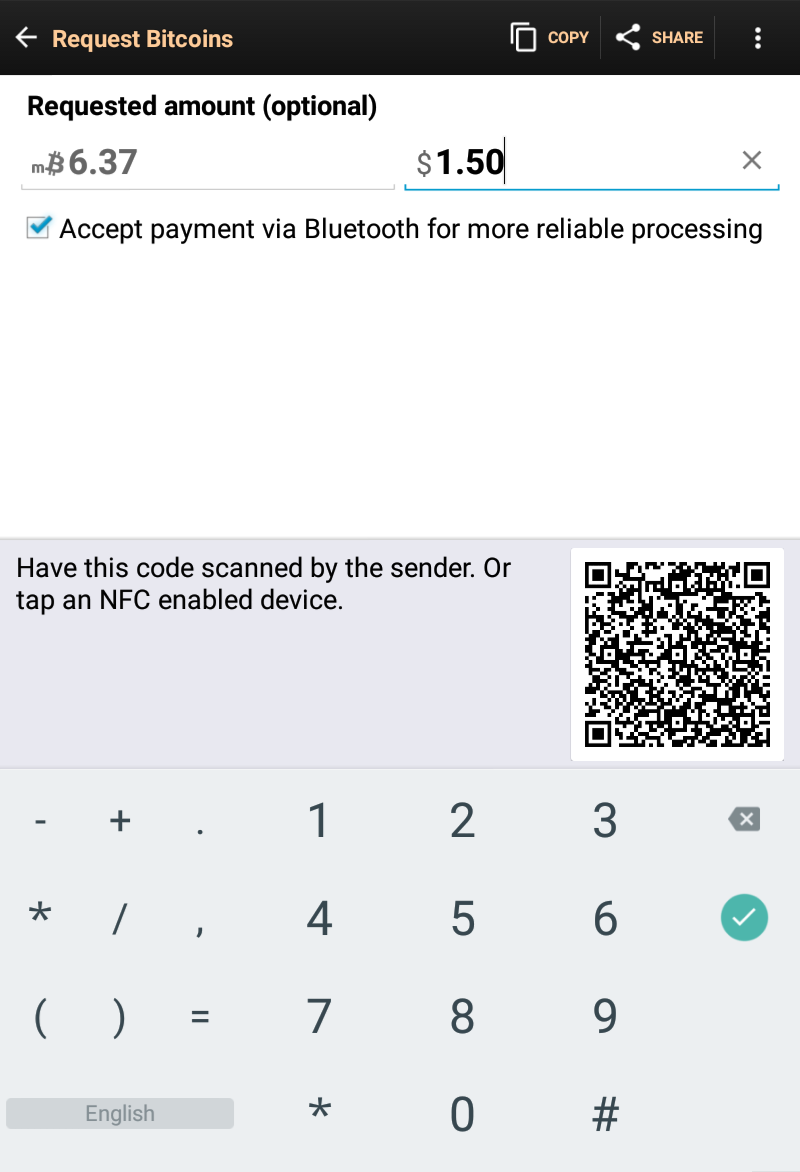
\includegraphics[width=0.6 \columnwidth,keepaspectratio]{figures/wallet-receive.png}
    \caption{A Bitcoin mobile wallet displays a QR code to receive money. The QR code encodes
             the receiving address (public key) and amount requested.}
    \label{fig.wallet-receive}
\end{figure}

Typically a wallet will be responsible for multiple
such pairs. In fact, the wallet may decide to generate a new private and public key pair occassionally,
and add it to its set of keys.

A primary job of the wallet is to know how much money it holds.
The wallet remains in contact with its full node and becomes aware of the evolving UTXO set. It
can find out how much money it owns by walking the UTXO set and inspecting it for outputs that correspond
to public keys in its set. The value held by a wallet is simply their sum:

\[
  v = \sum_{\textsf{out} \in \textsf{UTXO}} \textsf{out.v}
\]

This can be displayed to the user as \emph{``Your balance''} and, naturally, may change over time
as money is received (and new UTXOs are added to the set) or sent (and old UTXOs are consumed from the set).

\begin{figure}[h]
  \centering
  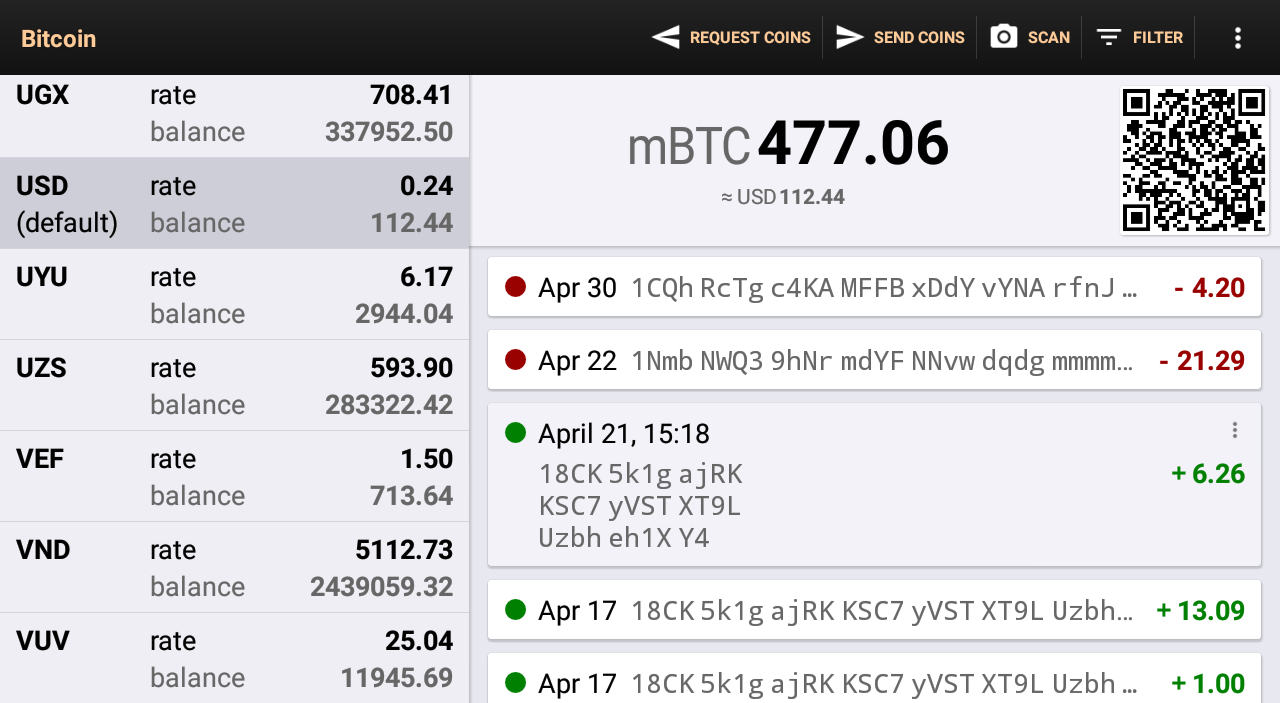
\includegraphics[width=0.9 \columnwidth,keepaspectratio]{figures/wallet-balance.png}
  \caption{A Bitcoin mobile wallet prominently displays its current balance. The history of transactions
           received and sent from the wallet is also displayed underneath.}
  \label{fig.wallet-balance}
\end{figure}

So far, it may have seemed peculiar that everyone maintains the ledger containing everybody's transactions.
How can there be any privacy in a blockchain system if everyone knows everybody else's balances? A basic
privacy protection stems from the fact that the balances on the blockchain belong to \emph{public keys}
and not human identities. And yet, consider the case where the wallet uses only a single public key for
receiving all of its payments. Then two different senders could talk to each other and corroborate the
address of a receiver. For example, if a person receives payment for services from their employer, but is
also selling goods online and receiving payment for them, then the employer who is also a buyer of these
goods could readily deduce that their employee is the seller, a potentially undesirable linkage for the
employee.

For this reason, a well implemented wallet will generate a new public key
every time it needs to receive a new payment. That way, if the same wallet receives money from two different
sources, these sources cannot trivially deduce that they are sending money to the same receiving wallet, even
if they talk to each other. The way this is done is as follows. The wallet talks to its full node and retrieves
all the past transactions that have been recorded in the blockchain since genesis. If there exists a public key in the set
$\mathcal{PK}$ that does not appear in any past transaction, this public key can be displayed to the user for
receiving money. More precisely, the set of keys that have not been used and are available for receiving money
is $\mathcal{PK} \setminus \bigcup \{ \tx\textsf{.outs} \}_{\tx \in txs}$, where $txs$ denotes all past transactions
recorded on chain.

Otherwise, if this set of keys is empty, a new key pair is generated by invoking $Gen(1^\kappa)$ again anew.
The newly generated key pair is then
appended to the set $\mathcal{PK}$ and displayed to the user. Until this key becomes used by a transaction recorded
on the blockchain, it will not be rotated again, but it will keep being displayed all the same. This means that
a particular receiving address can still be reused if the receiving user hands over the receiving address to one
payer and immediately hands over the receiving address to a second payer, before a transaction from the first payer
has made it to the blockchain. Yet, this provides significantly more privacy than a wallet that does not rotate
keys.

When a new transaction that pays into one of the public keys in $\mathcal{PK}$ is detected on the mempool, the
wallet displays a notification to the user that a payment has been received, together with the amount received.
This payment is displayed as \emph{unconfirmed} until the transaction is included in the longest chain and is
buried under a sufficient number of blocks. At this point, the transaction is displayed to the user as \emph{confirmed}.
The number of blocks required until a transaction is confirmed is a parameter that each wallet can choose differently,
depending on their desired security guarantees. While the transaction is becoming confirmed, the user is informed
of how many blocks have been mined on top of the transaction so far in order to indicate some kind of progress.

\section{Sending Money}

When the time comes for the user to spend their money, the user clicks on a different button in the wallet that
allows them to input a receiving address (or scan a QR code) and an amount of money to send.

{\color{red} more on sending money... }

\section{Online and Offline Wallets}

{\color{red} online and offline wallets...}

{\color{red}
\begin{itemize}
\item Online and offline wallets
\item Wallet seeds
\item Hardware wallets, brain wallets
\item Hierarchical Deterministic wallets
\item Collecting UTXOs to create a new transaction
\item Knapsack, minimizing fees
\item Privacy -- tracking transactions, associating addresses
\item Creating new addresses for privacy reasons
\end{itemize}
}
